\documentclass{cmspaper}
\begin{document}

%==============================================================================
% title page for few authors

\begin{titlepage}

% select one of the following and type in the proper number:
   \cmsnote{2005/TBD}
%  \internalnote{2005/000}
%  \conferencereport{2005/000}
   \date{\today}

  \title{DRAFT Technical Design of the Dataset Bookkeeping System DRAFT}

  \note{Draft Version v0\_7}

  \begin{Authlist}
    M. Anzar Afaq, Lothar Bauerdick, Greg Graham, Vijay Sekhri, Igor Terekhov, 
    Yujun Wu
       \Instfoot{fnal}{Fermi National Accelerator Laboratory}
    Lassi Tuura
       \Instfoot{ne}{Northeastern Unversity, Boston, MA, USA}
    Peter Elmer
       \Instfoot{prince}{Princeton University, Trenton, NJ, USA}
    Tim Barrass
       \Instfoot{bristol}{University of Bristol, Bristol, UK}
  \end{Authlist}

\collaboration{for the CMS collaboration}

  \begin{abstract}
      This note describes the Dataset Bookkeeping System (DBS) prototype for the 
  CMS Data Management (DM) project.  The DBS will
  store information about real and simulated CMS data in a queriable format.  The
  supported queries will allow users and their agents to discover avaliable 
  data, to retrieve further information about specific data, and to 
  derive analysis datasets. This note contains some use cases and requirements
  for the DBS.  The technical design of the DBS is presented.
    \end{abstract} 

  
\end{titlepage}

\setcounter{page}{2}%JPP

\section{Introduction}
\label{sec:intro}

The Dataset Bookkeeping System (DBS) part of the CMS Data Management system
provides the means to discover, define and use for processing CMS event data.
It tracks primarily {\em datasets} and their associated attributes.

This document describes the concepts used by CMS in data management and
specifies the bookkeeping system in detail that is sufficient to build the
baseline data management system described elsewhere~\cite{dmman}.  We begin
with a description of the CMS data organisation by expanding on the work of
the Data Management RTAG~\cite{rtag7} and the CMS Computing Model\~cite{CM}.
This is followed by a set of scenarios illustrating the primary uses of the
bookkeeping system.  Finally we provide a mapping of the organisational
concepts to relational database entities followed by an architectural
description of the components making up the bookkeeping system.

Access to CMS data should take place through interfaces designed for an 
appropriate level of abstraction for the end user.  The system will not require 
knowledge of implementation details, such as files or transport mechanisms. 
The dataset bookkeeping system (DBS) will take advantage of external infrastructure where 
possible.  The design will occasionally make 
reference to external databases or systems as required.  The DBS will 
concentrate on supporting the decomposition of datasets into event collections, 
finding the 
components needed to analyze or to transfer an event collection, and the making 
attributes available to support a sensible level of dataset discovery service.  


%It was taken as an operating assumption that POOL can be considered to be a service that 
%exists for the duration of a running application only.  The DBS may contain POOL contact 
%information, but will not rely on POOL itself to run queries or for replica information.

\section{Refining the Data Organisation}

\begin{figure}[hbtp]
  \begin{center}
    \resizebox{10cm}{!}{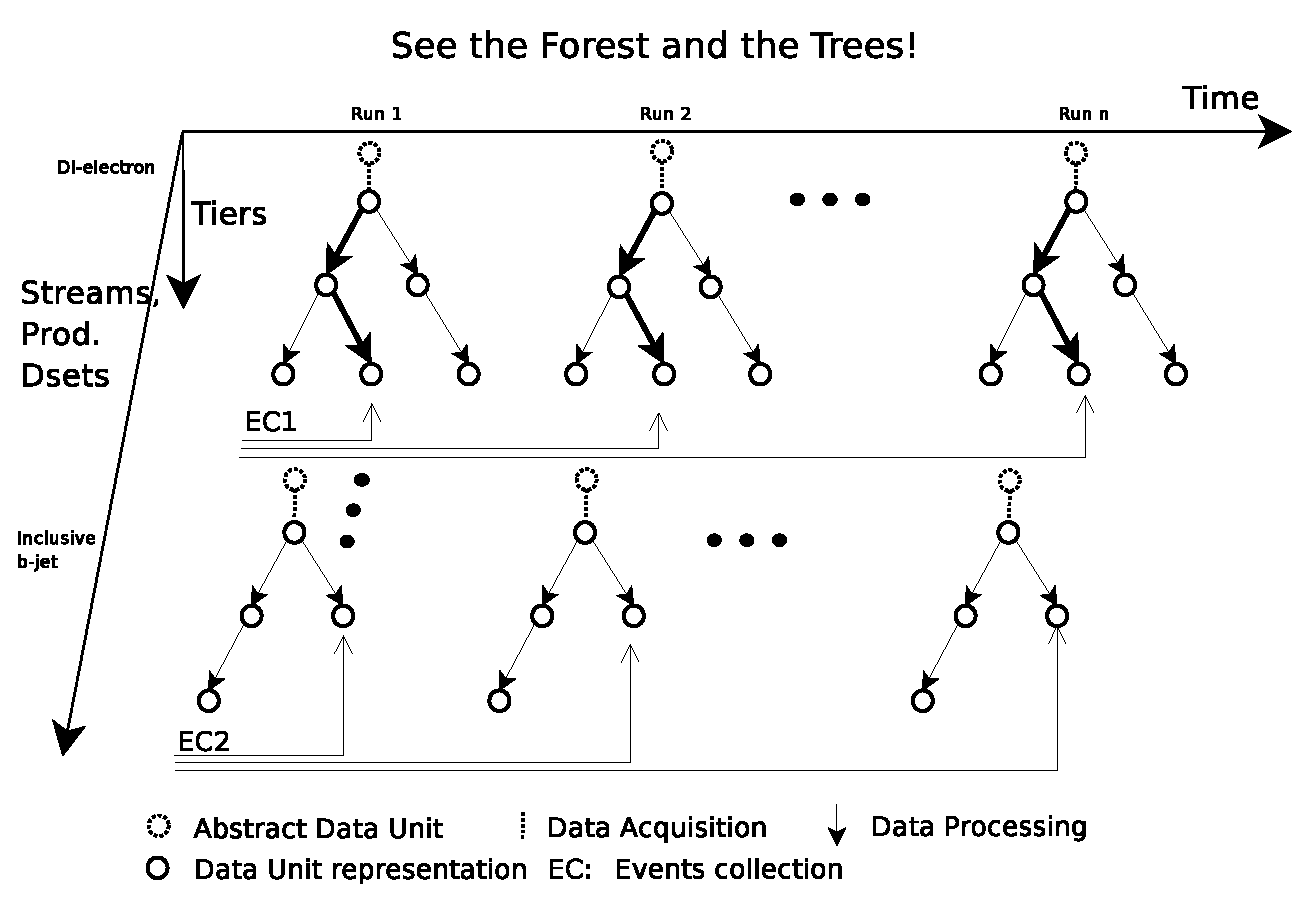
\includegraphics{forest.eps}}
    \caption{The figure shows a forest of trees.  The root of each tree is a 
chunk of data defined by some criterion, such as run number and trigger condition.
The path to each node in the tree represents the result of processing that 
data through a particular sequence of processing steps.  Each node is called 
a ``data unit representation''.  There can be trees in different Primary Datasets (along the 
axis pointing out of the page) and there can be Event Collections comprising nodes 
within each Primary Dataset that have the same processing path. An Event Collection 
that contains all possible like-path nodes in a Primary Dataset is a Dataset 
Representation.}
    \label{fig:forest}
  \end{center}
\end{figure}

We following terms define the organisation of CMS data:

\begin{itemize}
\item {\bf (Online) Stream}.  A stream is the largest unit of data organisation
and can be thought of as a collection of the output event data from the CMS
detector grouped by sets of high-level triggers that ``go together'' for
analysis purposes.  [FIXME: The bookkeeping system is not directly concerned
with online streams, except as means to narrow down to interesting primary
datasets.]

\item {\bf Primary Dataset}, also Production Dataset.  The main
data management concept: the unit of data accessed to analyse a given trigger.
Discovery and delivery of data is mainly concerned about production datasets.
CMS expects to have of the order of 50 production datasets.  Primary datasets
comprise data generated with the same parameters for Monte Carlo data.

\item {\bf Data Tier}. Type of content and degree of processing applied to the
data: {\em RAW} The raw event data written by the filter farm; {\em RECO} All
reconstructed data coming from the production engine; {\em FEVT} RAW + RECO;
{\em AOD} [FIXME].

\item {\bf Processed Dataset}. This is a selection of data from a Primary Dataset
defined by the exact processing history applied to it.  For example, the reconstructed data
is a {\em processed dataset}, namely it is the result of processing the raw data.
Key parameters defining a processing include the primary dataset, data tier,
processing pass number, program configuration [FIXME: algorithm parameter set
ids], calibration version.

\item{\bf Event Collection}. The smallest subset of a Processed Dataset that
user is able to access through the bookkeeping system, i.e. without using an
analysis application.  It maps to one or more files.  A ``run'' may be an
event collection for instance.

\item {\bf Analysis Dataset}.  A subset of a primary dataset, i.e. a set of
event collections.  Many useful entities are expressed as Analysis Datasets, 
such as the results of a skim or a managed block of data.

\item {\bf Events}.  The data from a single crossing.  Events are not managed
or accessible as such; one must use a data processing application to access
detail below an event collection.
\end{itemize}

We present these entities in Figure~\ref{fig:forest} and their relationships
in Figure~\ref{fig:highlevel}.  The figures express the information model
for the bookkeeping system, not the actual schema we will use.
The mapping of the information model into a schema is discussed in more
detail in section~\ref{details} after we have listed some primary use
cases.  A more precise definition of these entities in terms of subsets of
the data appears in the Appendix~\ref{appendix}.

\begin{figure}[hbtp]
  \begin{center}
    \resizebox{6cm}{!}{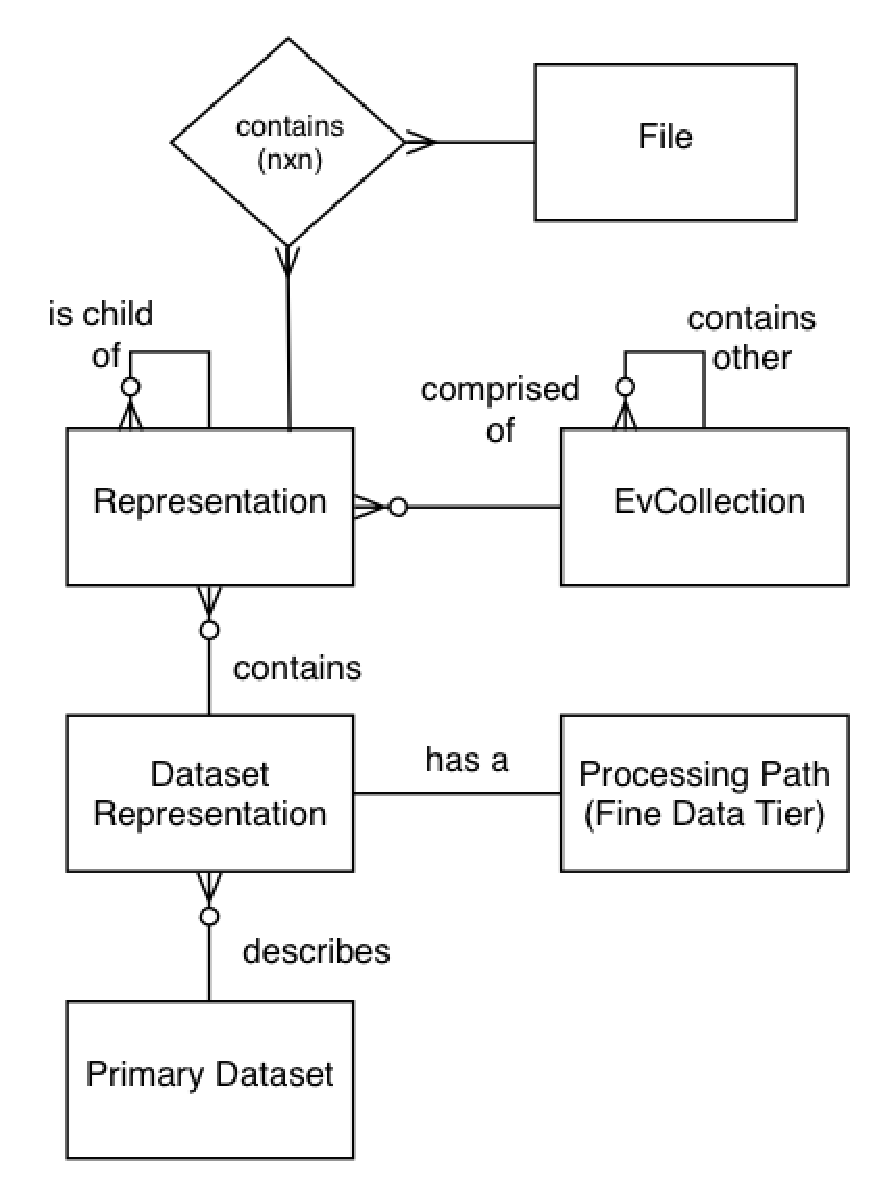
\includegraphics{DatasetBookkeeping-1a.eps}}
    \caption{Basic outline of the core DBS schema including the basic entities outlined 
in the Introduction: Primary Dataset, Dataset Representation, Representation, 
and Event Collection.  A few other supporting entities are shown as well.  Representation 
is mapped $N$ to $N$ with Logical Files. }
    \label{fig:highlevel}
  \end{center}
\end{figure}

\section{Implementation Concepts}

The Dataset Bookkeeping System contains the following implementation concepts 
that will be hidden from the users.  

\begin{itemize}
\item Files.  The DBS contains names of logical files.  It is not yet
determined how much file level metadata will be tracked by the DBS. 
\item Sites.  The DBS contains names of participating CMS sites that 
will host CMS data.  
\item Blocks.  The DBS contains Blocks as special aggregations of Event 
Collections. Blocks are aggregations with respect to underlying 
infrastructure parameters optimized for efficient storage and transfer.  
\end{itemize}

The DBS will treat special files, such as ``META'' files, in 
exactly the same way as all other logical files.  Special files that 
appear in more than one Event Collection will appear in more than one
relational row.  However, the EDM group will 
make changes in the way data is written in CMS so that the number of 
such special files tends to zero in the long run.  


\section{Scenarios, Use Cases, and Example Queries}

In this Section, we explore data import
({\em putting} data into the system), queries ({\em seeing} what is there),
and workflow for read access ({\em getting} data out of the system).

\subsection{Data import}

Data will be imported into the system in terms of the 
Event Collection entity.  

%Even though data will be produced one file at a time, its import  
%into the data management system is probably best done in terms of the 
%more abstract Event Collection entity. We imagine the 
%following scenario to put  a Event Collection 
%into the system in such a way that supports streaming.

\begin{itemize}
\item An agent is in possession of a file or files associated with an Event Collection
containing real data.
\item The agent utilizes an API method addToDataset(*evCollInfo).  The evCollInfo structure 
will contain information like 
\begin{itemize}
\item Logical Filenames associated with the import
\item Attributes associated with the production of the Event Collection, 
including the latest processing step and the input Event Collection(s). 
\end{itemize}
\item The method searches for the best block to which to add the Event Collection.  
The ``block'' is a special Analysis Dataset envisioned for this purpose.  
\footnote{Blocks will have attributes of interest to a data transfer and storage 
system, like maximum size and location information. These are of system interest only.}
It should reconcile the processing history with existing processing paths and 
open a new Processed Dataset if necessary.
\begin{itemize}
\item If there is an open block, the Event Collection is added to the open block.
\item If there is no open block, a new open block is created and the Event Collection is added to that one.
\item If the new block size is greater than the maximum block size, then the block is closed.  
\end{itemize}
\end{itemize}

Open blocks should not be transportable since that implies a complex wide area synchronization 
system. Streaming is of obvious concern here, and there is a tension between wanting to keep 
the blocksize small enough so that 
new data can be transferred to interested sites quickly and large enough to satisfy 
the needs of data management.
Alternatively, data can be streamed file by file; but in that case we need to synchronize
open blocks between sites sharing the particular data.

\subsection{User Queries}

Below we explore user queries corresponding to the various access modes,
and subsequently attempt to generalize. Among the goals of this section
is clarification of the role of a ``run''.

\subsubsection{Use case 1: Detector Expert}

  The first use case for selecting on run is doing detector studies, calibrations
and data quality. This use case does not address the time-varying 
calibrations/conditions are stored and accessed by applications from the 
conditions database itself, but merely how someone doing such studies would 
find the event data to do such studies. The common paradigm in HEP to access 
data through runs.
\begin{itemize}
\item An expert coming in the morning, reading the logbook sees that there was
     some problem with their subsystem overnight in run NNN; for example, if a crate 
     tripped off or was in some strange state, or oddities were seen in some 
     monitoring histogram, etc. Then the expert wants to look at some raw or 
     reconstructed data with some specialized application to learn more about the
     run quality or problems, often to classify it in a data-quality sense.
\item The detector expert at some later date may try to determine
     some calibration constants or corrections. Also in this case it will be natural
     for the expert to ask for different types of data, most typically with
     run ranges. Often what they do may include one component of actually 
     trying to break up the data into run ranges based on the problems and
     state of the detector and one component of actually determining the
     calibrations. 
\end{itemize}

"Run" here represents a natural quantum for thinking about the problem and
the DBS will be asked for data in these terms. Two implications are:
\begin{itemize}
\item The DBS will be asked for data at any tier from particular
    primary datasets with "run" as a selection. This has to be supported and
    some means of configuring jobs at this granularity for at least these
    categories of data must be provided.
\item "Data quality" attributes are likely 
    to be specified with a granularity of a single run. These flags may be
    specified for all data tiers of a particular run's data or just
    for particular ones. 
%    (As part of the discussions of the details of how
%    "run" is defined, DM should bring this point up explicitly. As it is a 
%    relatively common model in HEP, we can probably assume it for the moment.
%    See below for further details.)
\end{itemize}

Runs can be represented as Event Collections, and run numbers can be stored 
in a metadata support table going along with Event Collection.  Querying on 
run number amounts to first querying on attributes that can identify a 
Primary Dataset and a history of Processing.  Then by providing the set of 
interesting run numbers the corresponding Event Collections can be found.

The fact that data is accessed by "run" does not imply that the 
calibrations or conditions need to fall on run boundaries.  Up to a few 
parameters of interest for querying, these are usually 
read in bulk by applications so that there is no need to track these in the 
DBS.    Simple attributes like Run status flags 
can be stored in the DBS and later queried 
if they are imported along with the Event Collections.
Similarly data quality decisions with a finer granularity than 
run will be handled by an external conditions database and require 
the use of an application for access. 

\subsubsection{Use case 2: Production}
\label{sec:UCprod}

  The production system typically takes an Analysis Dataset or Processed Dataset
as input and processes it to produce a processed representation the input, or 
another Analysis Dataset or Processed Dataset. This use case includes reprocessing
and Monte Carlo production.

%  So how are "runs" sometimes used here? 

\begin{itemize}
\item The input Analysis Dataset is specified by a run range or list
     of runs, most likely made by selecting on data quality attributes set by
     someone like the expert of use case 1.  
%\item If the output is intended to be selectable with a run granularity,
%     the production system may process a given dataset by 
%     breaking it up into individual pieces with a granularity such that
%     the run genealogy of each output can be followed back to an input.
\end{itemize}

The user may be interested in tracking two types of "history" here:
\begin{itemize}
      \item macro level: how one dataset was transformed to another
      \item micro level: how one "run" representation is mapped to anther one
\end{itemize}
The first is tracked by explicitly including the processing path in the
definition of an Event Collection as represented internally in the DBS.  
The second is tracked by maintaining a relation between Analysis Datasets
and Event Collections.

The use of run ranges and/or run lists explicitly to define the input is 
partly incidental. If the goal of the production system is seen as
processing one dataset into another, the run-ranges and/or run lists 
should be captured explicitly in the DBS as an Analysis Dataset. 
%I would claim that the proper 
%concept for capturing this is a "dataset" (e.g. as some sort of "dataset 
%tag"). 

If the output is intended to be queryable by run number, then the production 
system may process the input dataset by breaking it up into runs.  This is the 
easiest scenario to envision because the processed runs can then be stored 
directly back into the DBS and aggregated into an output Analysis Dataset such
that input runs and output runs are in one to one correspondence.
However, even the hard case involving splitting and merging can be represented here. 
See section \ref{sec:createEvColl} for more information. 
The production system is explicitly collaborating in propagating the
"run" granularity from input to output.  It can choose any granularity it 
wishes as long as it is tracked by the DBS.  

Otherwise, this use case is supported in much the same way as the previous one.  An input 
Primary Dataset and input processing path is given, and then all Event Collections
matching the run range can be retrieved.  When tracking the processing
taking place within a Primary Dataset, even if the framework does not track processing
of individual Event Collections within an Analysis Dataset, the Event Collections 
may be loaded into the DBS anyway.  This preserves the structure of tracking 
the processing paths through Event Collections, and the set of 
files corresponding to the whole processed Analysis Dataset can be assigned to 
each Event Collection in the derived Analysis Dataset.  

\subsubsection{Use case 3: Analysis End-user}

  The analysis end-user will process Analysis Datasets for more
than one run through some application such that the output no longer has
a 1-1 mapping to run. See section \ref{sec:createEvColl} for an 
explanation of how such filter and skim output can be 
represented in the schema.
\begin{itemize}
\item The detector expert is still working and may decide, after the 
     analysis-user has already run their analysis over a dataset, that a
     particular run was "bad" after all and should be excluded from their
     end result. 
\item The detector expert or analysis group may provide some set of
     corrections/updates which the analysis-user needs to apply themselves
     For example, constants that arrive too late to be included in 
     the last re-reconstruction or AOD production step, or were 
     actually generated from the output of
     the last re-reco or AOD production step. 
\end{itemize}
The DBS and DM should be involved in tracking Analysis Datasets in which
some mangling has gone on with respect to runs and the relationship of 
the resulting Event Collections to runs becomes significantly more complex.

In the case 
where multiple jobs are doing the processing, the DBS should also be able
to keep track of which expected data units have been imported successfully and which 
have not.  In the case where there is only output product Analysis Dataset, 
then it is still useful to be able to query and find out which component
input Event Collections, it doesn't matter were processed to 
arrive at the desired result.  This is important to be able to track important 
aggregte dataset properties like luminosity.

\subsubsection{Support for Generalized Queries}

%The following queries can be covered in the proposed schema.  In most cases, the 
%queries are straightforward in light of the proposed schema.  As with the diagrams, 
%joins with support tables are omitted in the following for clarity.

Each of the following queries are listed with a short plan for resolving the query.
(This section to be fixed later.) 

\begin{itemize}
\item Find all files associated with a Primary Dataset.  Compound join on Primary
Dataset, Processed Dataset, Event Collection, and File.
  \begin{itemize}
  \item Find all files associated with a run.  Simple join on Event Collection, File and selection for run number.
  \item Find all files associated with a block.  Compound join on Analysis Dataset, Event Collection, 
and File.
  \end{itemize}
\item Find all Analysis Datasets associated with a Processed Dataset.  Filtered selection on 
simple join on Analysis Dataset, Event Collection. (This query caused us to consider that runs 
must belong to distinct datasets, or equivalently that the unique attributes of 
run must include at least both run number and dataset id.  If it is not so, then 
these types of queries become much more complex.)
  \begin{itemize}
  \item Find all assignments associated with a Monte-Carlo Primary Dataset. Filtered selection on join.
  \item Find all blocks and block locations associated with a Processed Dataset. Filtered selection 
  on simple join.
  \end{itemize}
\item Find all data. Unfiltered selection on Primary Dataset.
  \begin{itemize}
  \item Find all data matching a physics criterion.  Filtered selection on dataset or 
  on simple join on dataset, run.
  \item How many are runs in a Processed Dataset.  
Cardinality of simple join on dataset, Event Collection and selection on run number.
  \item How many events in a dataset.  Selection on dataset.  (This query caused us to 
  consider keeping track of bulk properties such as total number of events that could be 
  updated every time a run is imported.  This could work for luminosity and cross section too.)
  \item Find digitized data corresponding to specific generated data. 
  Filtered selection on Processed Dataset or compound filtered selection of the join of 
Analysis Dataset and Event Collection.  
  \end{itemize}
\end{itemize}

\subsection{Defining derived datasets}
%%
%A user will be able to define new Analysis Datasets. 
%Some of these datasets will represent the results of processing
%of an entire production dataset and will be done on behalf of the entire
%collaboration. Others will be defined by groups. Finally, ``private''
%datasets defined by individual users for their own consumption may be
%supported. We say that such user-defined (aka analysis, aka derived)
%datasets have a {\em scope} associated with them.

(This section to be fixed. Existing content was subsumed into the above sections.  
New content should include discussion on snapshots and defining datasets by 
query that we had on March 22.) 

%Some of these derived datasets will also be ``filters'' of their parent
%datasets, where the one-to-one relation between a parent and a child
%event (representation) is not preserved. It shall therefore be possible
%to mark such filtered datasets (sometimes called {\em skims}) appropriately
%when defining them.
 
\subsection{Workflow scenario}

The following workflow building scenario explores the 
interface between data management and workflow management.
\begin{itemize}
\item A physicist or agent creates jobs based on data identified by queries against 
the DBS.  A handle to an Analysis Dataset containing a number $N$ of
Event Collections is returned.  
\item The physicist or agent creates $M <= N$ jobs.  The agent may create jobs with more than 
one Event Collection per job if optimization works out that way.  The job 
creation tool creates jobs in a site independent fashion, knowing only about site 
independent dataset parameters, input event collections, etc and instructions for 
connecting to the data.  (eg- a POOL catalog connection string.)
\item Physicist or agent submits jobs.  Job submission tool consults the DRS through the 
application layer.  Information about sites where the data resides is obtained 
now.  An algorithm, round robin for example, assigns jobs to sites based on where 
corresponding blocks are located.
\item Job files are transferred to the execution site along with the job using e.g. Phedex.
\item The jobs are 'localized' upon transfer to the site.
\item Output data is created and transferred by SRM to the final resting place.
\item The output data is published into the DBS.
\end{itemize}

\section{The Entities and Relationships}

The DBS keeps track of some implementation details in the backend, such as 
Fil or Site.
The schema proposed here has a progressive view of abstraction 
with implementation specific objects at one end, and primary datasets at the 
other end, and 
intermediate abstractions between them.  The user is presented with the most
abstract concepts first, and consciously has to drill 
down to get to the progressively less and less abstract objects like 
logical file names if he/she desires.  Mostly these objects will be covered by the
API.  The detailed ER diagram is given in Figure \ref{fig:detailed}. We 
would like to first go over the core entities introduced earlier and
shown in Figure \ref{fig:highlevel}.

\subsection{Basic Entities}

At the base is the Primary Dataset.  
Following the definition in section \ref{sec:intro},  
attributes that define the kind of data contained in the 
primary dataset, such as generation parameters for Monte Carlo or 
trigger bit information for real data, are included here or in a 
Primary Dataset support table.  

The Processed Dataset is obtained by 
selecting out of the Primary Dataset a particular subset of the data that has been 
processed by a given sequence of application steps.  The sequence is stored 
in the supporting entity Processing Paths.  For example,
if a chunk of raw data were processed first by a filter program P1 followed 
by a reconstruction program P2, then the processing path is /P1/P2, up to how we
store information about the symbols in the path, of course.  Each component 
of the path may contain a reference to a distinct record of the 
invocation parameters and the corresponding application and version that did 
the processing\footnote{This is a fine grained example of what is sometimes called
``Data Tier''.  The Data Tier typically contains only information about kind
of application was run.  This has been generalized to contain much more information 
about the processing path.}. 

The Event Collection is a well defined result set of data obtained by processing a 
well defined input chunk of data through a given Processing Path.  (See figure \ref{fig:forest}).
It is also the smallest abstract entity that can be mapped to a specific set of files.

The figure shows that a Event Collection can refer to other Event Collections.  This 
supports directly the following two cases: 
\begin{itemize}
\item The Event Collection contains a reference to its parent. 
\item The Event Collection may contain references to more than one 
Event Collection in the same processing tree.\footnote{Please see the definition of
Compound Event Collection in the appendix.}
\end{itemize}
The former case can be implemented directly by including the 
full processing path in the unique key of the Event Collection as well as the 
ID of the Primary Event Collection.  The second case requires an adjunct 
mapping table. 
If the user wants to create an Analysis Dataset consisting of both Hits and 
Digis data in CMS, then the latter construct would be useful.  

The Analysis Dataset is an aggregation of Event Collections.  Unlike the 
Processed Dataset which must contain all of the Event Collections at a 
particular Processing Path, the Analysis Dataset flexibly contains any subset
thereof.  Please see the appendix for a precise formulation.

Although the CMS framework makes no distinction between Analysis Dataset and Event Collection, 
it is wise in a relational database to make such a distinction.  The former is just normal aggregation
of objects into sets while the latter is specifically needed to track the implicit
OO relationships that are possible in the data itself
but not in an RDBMS. These relationships are tracked by including the processing path in the 
Event Collection in the sense that each application is concerned with specific objects in the 
event tree.  

The Analysis Dataset refers to itself to support
the use case of one user adding to the Analysis Dataset of another user.  Again, this
may be implemented by a simple mapping table.

The Processed Dataset has a special relationship to Event Collection (non-Compound) 
in that the primary key attributes 
of Event Collection flow through the Processed Dataset.  This does not occur 
with Analysis Dataset in general, and hence it is called out in the diagram.
Furthermore it should be possible to characterize and
create a Processed Dataset before adding a Event Collection to it.  

The File enitity is in a many to 
many relationship with representations.  It is intended that special files 
like the CARF ``META'' files can belong to more than one Event Collection.
The META files are a contemporary implementation detail of the EDM, 
and the DBS will not track them differently from other files.  
As the EDM improves in this 
respect, the DBS will not have to adjust.

The progressive relationship of the entities allows queries 
premised upon physics attributes on the Primary Dataset side 
to be naturally drilled down by the system into queries about 
files without specific user involvement.
The structure also provides a natural heirarchy of categories within which to organize the 
attributes according to their abstraction.  

\subsection{Adding More Detail -- Relations and Constraints}

%The schema above captures the basic idea of what the DBS is trying to achieve.  
%One can build upon this to obtain a more detailed picture that includes
%external linkages and some basic method of blocking the data 
%together into manageable pieces for transfer and storage.  This leads to the 
%enhancements found in Figure \ref{fig:detailed}.

The fundamental unit of data import into the system is the Event Collection.  A Event Collection 
can correspond to a run or any other chunk of data that is considered fundamental and can be 
mapped to a set of files\footnote{The set of files in one Event Collection are allowed to overlap with 
those in another Event Collection.  This accommodates metadata files, for example.  This 
aspect can be tightened later as the EDM evolves.}.  
A special kind of Event Collection is the Primary Event Collection.  The Primary Event Collection
corresponds to the root node in a processing tree of figure \ref{fig:forest}.  This entity
will contain attributes associated with the whole tree, possibly these are keys into 
an external Monte Carlo request database or run conditions database.

Analysis Datasets can support different kinds of constraints depending on the 
subtype.  The block would be a partition on Processed Datasets, and would have a 
relationship to a site entity.  
\begin{figure}[hbtp]
  \begin{center}
    \resizebox{12cm}{!}{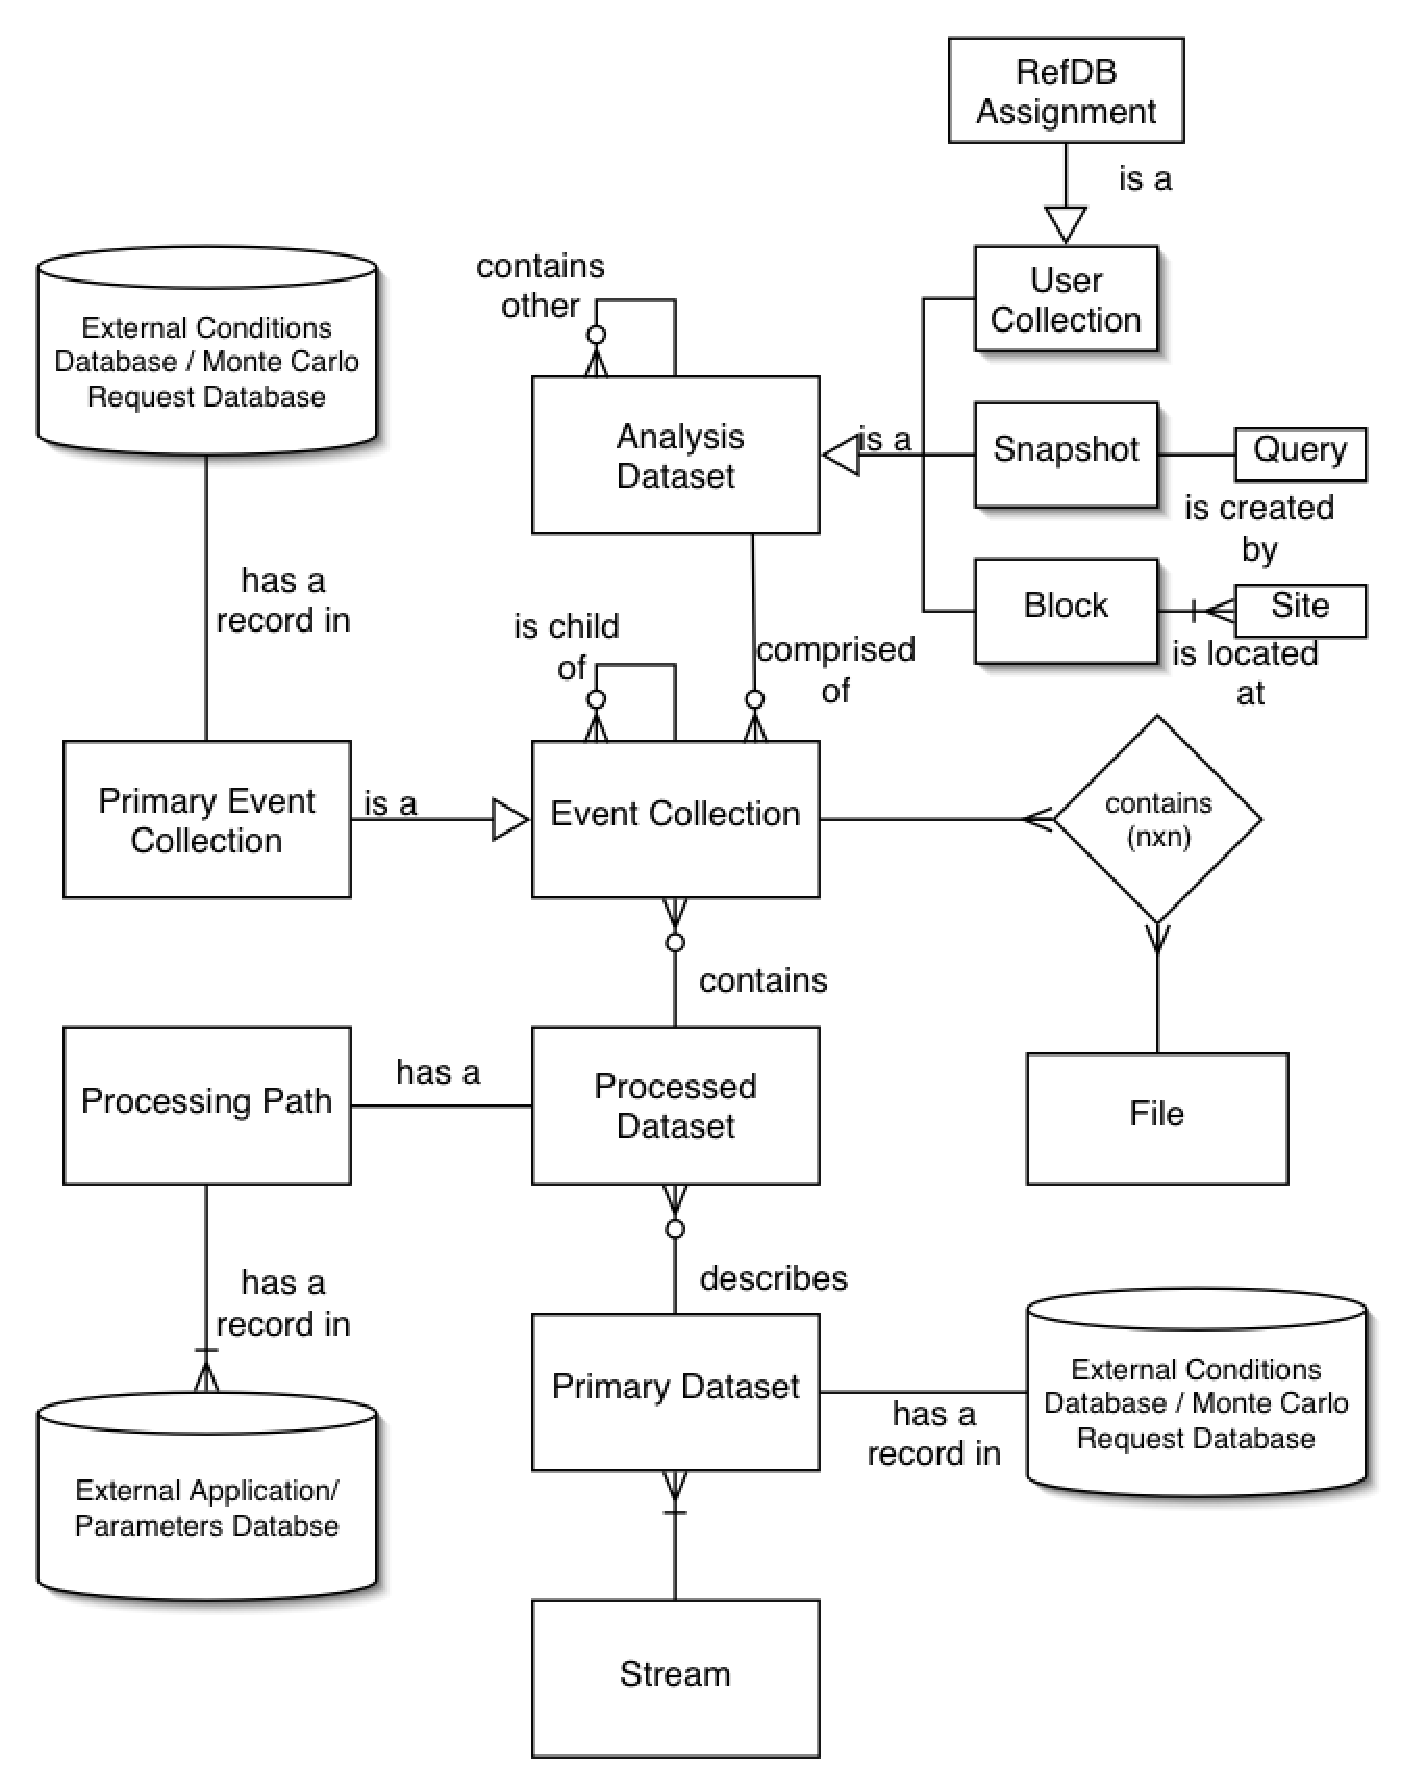
\includegraphics{DatasetBookkeeping-2a.eps}}
    \caption{A (nearly) complete schema.}
    \label{fig:detailed}
  \end{center}
\end{figure}
The block will aid in managing physical placement and storage of data.  
Blocks are therefore distinguished by having a one to many relationship to a supporting site 
entity.  Blocks satisfy the extra constraint that they  
partition the Processed Dataset\footnote{Technically, they partition the 
Processed Dataset in the sense that no event IDs
can exist in two different blocks.}.  This  simplifies the task of deciding which 
blocks to transfer given a set of interesting Analysis Datasets.

Blocks are special in that they represent a new implementation detail 
that must be hidden from the physicist.  However, block constraints and 
behavior can be hidden in the application layer.  Blocksize 
introduces a scale into the system,  however this can be addressed hierarchically 
through the self relation of Analysis Dataset
\footnote{If one introduces blocks in order to deal with data on a given scale, one someday may need 
to introduce "super-blocks" if that scale changes, and so on.}. 

User collections directly support the idea that users can specify 
collections of interest to them.  User collections list component Event Collections
and pre-existing Analysis Datasets and can span multiple blocks.  
envisaged.  The data associated with a RefDB production assignment can also be supported 
as a special kind of user collection.

A further specialization is the Snapshot.  The Snapshot is an Analysis Dataset whose results 
comprise the result of a query of the DBS.  The query itself is stored in a support table, and 
the cretion time is recorded.
The snapshot could be a closed set of Event Collections in a streamed dataset that does 
not change or grow as the dataset grows.  

\subsection{Even more detail -- tables and attributes}

The file entity contains obvious 
file attributes, such as logical filename, file size, cardinal times like creation and 
last access times, and checksum.  It does not contain site information or physical filename 
information.  Rather, replicas will be tracked externally.  

Event Collection will contain brief and essential attributes such as run number, 
number of events in the collection, cardinal times like creation and access times, 
and a run status flag.  Run conditions and calibration constants will
be kept in external databases.  Part of the primary key of the Event Collection
should be the Primary Dataset that the Event Collection 
belongs to as well as the complete processing path.  This should be a unique key of 
Processed Dataset.  

Blocks will have a unique block id that identifies its partition within its processed dataset.
It will have a block size and other low level attributes related to implementation.  Blocks 
will not contain physics metadata.  
Blocks will have a flag to indicate whether or not they are open for writing. 
In order to simplify the problem of locating blocks to sites, it is a 
requirement that open blocks be restricted to a single site\footnote{This has obvious 
implications for streaming, and can be later dropped or revisited when we review the distributed 
aspects.}.

The Processed Dataset will contain Primary Dataset and Processing Path 
references.
In addition, quantities that are determined to be "searchable" that are related to the 
specific level of processing of this data should be included directly here for 
users to query on.  

Analysis Datasets can contain further attributes.  User collections should for 
example contain annotations indicating why they were created.  Blocks contain 
pointers to sites.  Collections corresponding to assignment IDs will contain pointers 
into the RefDB plus some metadata for querying. Snapshots will contain references to the
text queries that created them.

Storage of attributes supporting the various 
entities  can be implemented as support tables when the actual schema is written down.  
The support table 
is a basic ER design pattern which allows metadata to be stored in a queryable format 
outside of the table directly representing the entity.  Attributes such as generation and 
simulation parameters for Monte-Carlo to run status information can be kept in support 
tables.   The support tables for the proposed schema have not been drawn for simplicity.  
Each principal entity in the schema should probably have a support table.

\subsection{Creating an Analysis Dataset from another Analysis Dataset}
\label{sec:createEvColl}

The input to a user Application is either an Analysis Dataset or an Event Collection.
We examine a few cases here to illustrate how these processing results can be 
recorded using the DBS schema.  Practically, the 
relation between Analysis Dataset and Event Collection 
(figure \ref{fig:highlevel}) is that the latter has an additional attribute that tells 
the application how to select out specific corresponding data from the former.  
In general we think of Event Collections being processed ino other Event Collections. 
But the results hold for Analysis Datasets too if we wrap the Input and Output Event Collections
in an Analysis Dataset where needed.

\subsubsection{Processing a Single Event Collection}

A trivial case is where the application input consists of a single Event Collection. 
This could be, for example, a single run.  The job processes the Event Collection 
and produces an output Event Collection, which is associated 
with newly produced files.  The new files are stored back into the DBS as a child 
Event Collection of the input.  

\subsubsection{Processing Multiple Units of Data in Parallel}

In this case, application input consists of an Analysis Dataset
comprising multiple Event Collections. This 
could be multiple runs for example.  If each component Event Collection can be 
processed by a single job\footnote{The processing is one to one input units to output 
units.  The technical condition here is that the processing 
of an input Event Collection produces a distinct set of files, up to a few common ``metadata'' files.}, then as in the above case of a single Event Collection, the results
can be piecewise stored back into the system as child Event Collections and then grouped
together to form an output Analysis Dataset.  

\subsubsection{Filtering or Skimming: Multiple Units of Input Data and Single Unit Output}

In this case, the application creates a single output Event Collection that is whole 
from many inputs. It is not practicable to subdivide the output 
Analysis Dataset in terms of whatever parameter
was used to index the input Event Collections.  For example, the input may be 
a list of runs and the output may be a single colletcion consisting of a few 
events from each run selected according to some physics criterion.  We 
assume that the output is a set of files for which there is no map
showing which files contain which events.  Then there are two choices.
\begin{enumerate}
\item Store the output back into the system as a single Event Collection with 
the output Analysis Dataset containing only that Event Collection as a new 
Primary Event Collection.   Some limited parentage information 
is kept in the form of a parent Analysis Dataset attribute
\item For each input Event Collection $i$, store the relation $(i,O)$ where 
$O$ is the output Event Collection.  In other words, the same set of 
files appears as the the output result of processing for each $i$.  This
would preserve all of the relationships and would 
result in more efficient queries.  
\end{enumerate}

\subsubsection{Reclustering: Multiple Units of Input Data and Multiple Mixed Outputs}

In this case, the application is accepting many input Event Collections
and producing split outputs that have no obvious correspondence to the 
inputs.  For exampe, the input could be 
an Analysis Dataset comprising Event Collections according to $N$ runs and the 
output could be an Analysis Dataset comprising outputs 
according to $M$ luminosity bins.  This is also called reclustering.
\begin{enumerate}
\item Store each reclustered Event Collection back into the system as a
primary Event Collection. 
\item For each input Event Collection $i$ and for each output Event Collection $j$,
store the relation $(i,j)$.  If it is at all known which specific inputs correspond to 
on output Event Collection,  the size of the set of relations can be cut down. 
In other words, the same set of 
files appears as the the output result of processing ranging over the input 
index $i$ holding the output index $j$ constant.  This 
preserves  all of the relationships and would 
result in more efficient queries.
\end{enumerate}



\section{Architecture}


At the top of the application stack is the application database server layer which contains
the application logic.  This layer abstracts the clients from the schema and is not 
to be confused with the database server proper such as Oracle which serves SQL requests.
The database server layer manages the API that user applications will see.  It needs to 
support basic use cases of queries against the underlying database, such as discovering 
datasets from metadata or asking for the number of events in a given run range.  It 
should also support an API to get the information needed to initiate an analysis.  

The dataset bookkeeping system (DBS) proper is kept immediately below the database 
server layer.  The dataset bookkeeping system was split into the "canonical" dataset 
bookkeeping system (DBS) plus a dataset replica service(DRS).  This reflects the 
desire to keep replica locating functionality out of the DBS altogether is possible, 
and in a separate schema if absolutely necessary.    We agreed that if fine grained 
site information was included, then access to site information (DRS) should be kept 
decoupled as possible from the actual core dataset bookkeeping functionality (DBS), 
hence the two interfaces in the diagram.  (This is a somewhat arbitrary distinction, 
and maybe it goes away upon further inspection.)

\begin{figure}[hbtp]
  \begin{center}
    \resizebox{6cm}{!}{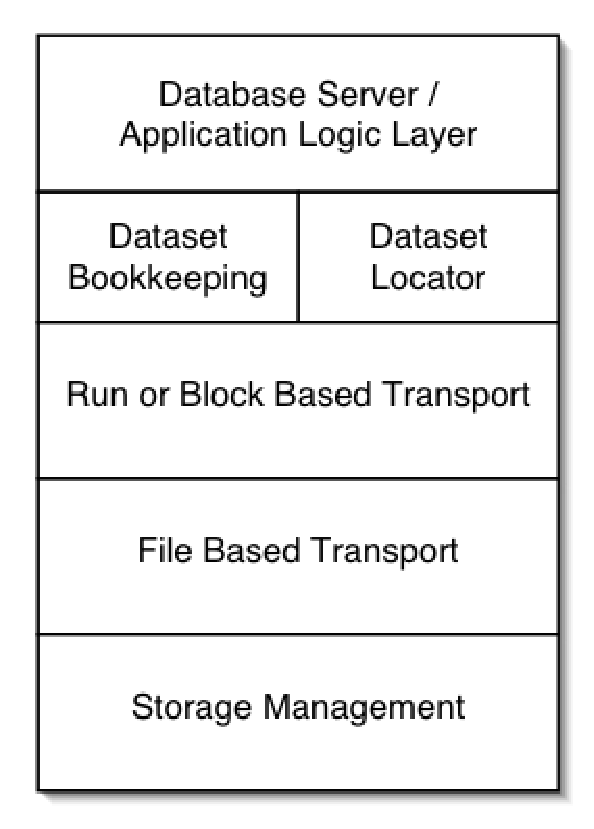
\includegraphics{DatasetBookkeeping-3a.eps}}
    \caption{}
    \label{fig:ex3}
  \end{center}
\end{figure}

Next, there is a layer specializing in Run and/or Block data transport.  
This layer can contain primitives and checks that guarantee transport of 
runs and/or blocks.  Underneath are file and storage infrastructure layers.

\subsection{Distributed Databases}

We did not explore the ramifications of distributing the database on the above schema.  
We briefly explored what it would mean to transfer a block to a site that was maintaining 
its own copy of the DBS.  We suspect that the corresponding runs would not have to be 
re-imported at that time.  Rather, we imagine that the corresponding data would be added 
to the local database through a lower level interface layer.  Important questions remain:  
is the block ID unique throughout all instances of a DBS?  What is the exact workflow for 
replicating a block?   After some discussion, we were nonetheless confident that the 
proposed schema with the addition of some transfer protocols would be sufficient.  
(To be expanded.) 

\section{Other Considerations}

Runs have a fill structure.  We do not at this time believe that substructure within 
runs need be tracked by this schema.  We prefer to imagine that a run conditions 
database will keep track of how run conditions change in a regular way taking into 
account a known fill structure.  Runs will change when irregularities occur and cause 
the operators to shut down the current run and start a new one.  

At this time, we do not foresee the need to create a dataset from a 
pre-existing Analysis Dataset.  In our current model, a dataset must be created 
before one can add data to it, and therefore all of the Analysis Datasets must 
already comprise data that belongs to a dataset.  


\appendix

\section{Addendum on Data ``Sets''}\label{appendix}

In order to clarify the relationships between the given entities given in the main part of 
this note, it was felt that some formulae would help. 

\subsection{Event Collections and Datasets}

\begin{enumerate}

\item {\bf A Primary (or Production) Dataset $\Delta$} 
contains all data that shares certain physics 
attributes such as trigger bits or generation channels.  For example, ``Higgs to 2 electron''
or ``W to e nu'' or some other physics channel or trigger or luminosity condition.  (We omit 
here an index spanning the roughly 50 various trigger bits/channels to be present in the 
real data.) 

\item {\bf A Processing Path $\pi$} is a sequence of applications with version imformation 
and invocation parameters that
characterizes the provenance of processed data.  The null path $\emptyset$ contains
no applications and represents ``raw data'' in the sense that it is unprocessed.  

\item {\bf A Processed Dataset $\Delta_{\pi}$} is a selection of data within a primary 
dataset $\Delta$ that contains only data that has the provenance $\pi$.  For example, 
``Digi data'' within $\Delta$ is $\Delta_{\mbox{Digi}}$.  Of course, the provenance specification 
can be as complicated as you wish.

\item Let $\Pi(\Delta)$ be the collection of all processing paths defined for a Primary 
Dataset $\Delta $.  Then 
\begin{equation}
    \Delta = \{ \Delta_{\pi} \mid \pi \in \Pi(\Delta) \}
\end{equation}

\item $\Delta_{\emptyset}$ refers to the raw data in $\Delta$. (Or unprocessed data for 
Monte Carlo data.) 

\item Let $\rho$ index units of data $\Delta_{\emptyset}^{\rho}$ 
in $\Delta_{\emptyset}$.  The unit 
could be a Monte Carlo run, it could be a raw data run, 
it could be a luminosity bin within a raw data run, 
individual events, etc.  Let $R(\Delta)$ be the 
set of all such indices in $\Delta$.

\item An {\bf Event Collection} $\Delta_{\pi}^{\rho}$ is the 
data in $\Delta$ that corresponds to the result of processing $\Delta_{\emptyset}^{\rho}$ 
through the given path $\pi$.  

\item The union
of all Event Collections of data units at some path $\Delta_{\pi}^{\rho}$ is 
\begin{equation}
\bigcup_{\rho \in R(\Delta)} \Delta_{\pi}^{\rho} = \Delta_{\pi}
\end{equation}
which is just another way of writing the Processed Dataset.  

\item An Event Collection $\Delta_{\pi}^{\rho}$ can 
be considered to be a node of data in a processing tree.  
The root node of such a tree is the {\bf Primary Collection} $\Delta_{\emptyset}^{\rho}$ 
of the unit of data.  The Primary Collection can correspond to a 
run of raw data, for example, or some other unit of data 
(other than a run) to be determined.  

\item The whole processing tree in $\Delta$ rooted 
at $\rho$ can be represented as $\Delta^{\rho}$. 
\begin{equation}
\Delta^{\rho} = \{ \Delta_{\pi}^{\rho} \mid \pi \in \Pi(\Delta) \}
\end{equation}

\item To get the Primary Dataset back again, 
\begin{equation}
\Delta = \bigcup_{\rho \in R(\Delta)} \Delta^{\rho} = \bigcup_{\rho \in R(\Delta)} \{ \Delta_{\pi}^{\rho} \mid \pi \in \Pi(\Delta) \} 
\end{equation}

\end{enumerate}


\subsection{Analysis Datasets}

And for Analysis Datasets, which are meant to be more flexible and user definable: 

\begin{enumerate}

\item Defining an Analysis Dataset as a collection of Event Collections of units of data.  
Consider some
subset $R_I$ of data indices of interest in $R(\Delta)$:  $R_I \subseteq R(\Delta)$.
Say one is interested only in 
data processed through some concrete path $\pi$.  An Analysis Dataset $\xi_{\pi}^{R_I}$
can be defined as 
\begin{equation}
\xi_{\pi}^{R_I} = \bigcup_{\rho \in R_I} \Delta_{\pi}^{\rho}
\end{equation}

\item Of course, one special case is a Processed Dataset. 
\begin{equation} 
\xi_{\pi}^{R(\Delta)} = \Delta_{\pi}
\end{equation}


\item Definition of a partition into $N$ disjoint $P_N$ on a set $X$ : 
$ P_N = \{ y_i \mid i = 1...N, y_i \subset X \} $ such that 
\begin{equation}
\bigcup_{i=1}^N y_i = X
\end{equation} 
and 
\begin{equation} 
y_i \cap y_j \neq \emptyset \mbox{ if and only if } i = j
\end{equation}
 
\item  Another special case of Analysis Dataset 
is for ``blocks'', or ``dataset partitions''.  For example, if
$P_N = \{ p_i \}$ is a partition over $R(\Delta)$ of size $N$, then : 
\begin{equation}
B_{\pi} = \{ \xi_{\pi}^{p_i} \mid i = 1...N\}
\end{equation}
is a set of ``blocks'' of data of type $\pi$.  For raw data, $\pi = \emptyset$.


\item Let $\Pi_J$ define some collection of interesting processing paths, like ``Hits and Digis'', 
in $\Pi(\Delta)$.  Let a Compound Event Collection $C_{\Pi_J}^{\rho}$ be defined by
\begin{equation}
C_{\Pi_J}^{\rho} = \{ \Delta_{\pi}^{\rho} \mid \pi \in \Pi_J \}
\end{equation}
In the E-R schema provided in the document, the Compound Event Collection is 
represented in the self-relation on the Event Collection entity.  We draw attention to 
this distinction here for clarity.

\item Defining an Analysis Dataset as a collection of compound Event Collections: 
\begin{equation}
\xi_{\Pi_J}^{R_I} = \bigcup_{\rho \in R_I} C_{\Pi_J}^{\rho} = \bigcup_{\rho \in R_I} \{ \Delta_{\pi}^{\rho} \mid \pi \in \Pi_J \}
\end{equation}

\item Blocks can be defined similarly over Compound Event Collections if the $R_I$ are a partition 
of $R(\Delta)$.

\end{enumerate}

All types of entities above can be represented in the provided schema.  (Or the schema
is in error.)  The Analysis Dataset can be understood as a cartesian product of some
``results of processing'' and some ``units of interesting data''.  


\begin{thebibliography}{9}
  \bibitem{dmman} The DM.txt document, being migrated into the Computing
      TDR (CTDR) document repository
  \bibitem{rtag7} {\bf CMS Internal Note 2004/038}, R. Harris et al., 
    {\it Report of the CMS Data Management RTAG}

  \bibitem{CM} {\bf CMS Note 2004/031}, C. Grandi, D. Strickland,
               L. Taylor, {\bf The CMS Computing Model}

  \bibitem {NOTE000} {\bf CMS Note 2005/000},
    X.Somebody et al.,
    {\em "CMS Note Template"}.
\end{thebibliography}
 
%------------------------------------------------------------------------------
\pagebreak

\end{document}
